% Isaac Dunn Part II Computer Science Dissertation
\documentclass[12pt,a4paper,twoside,openright]{report}
\usepackage[pdfborder={0 0 0}]{hyperref}    % turns references into hyperlinks
\usepackage[margin=25mm]{geometry}  % adjusts page layout
\usepackage{mathpazo}  % style
\usepackage{graphicx}  % allows inclusion of PDF, PNG and JPG images
\graphicspath{ {./figs/} }
\DeclareGraphicsExtensions{.pdf,.png,.jpg}
\usepackage{verbatim}
\usepackage{docmute}   % only needed to allow inclusion of proposal.tex
\usepackage{amsmath}
\usepackage{amsfonts}
\usepackage{algorithm}
\usepackage[noend]{algpseudocode}
\usepackage{enumitem}
\usepackage{color}
\usepackage{listings}
\usepackage{subcaption}
\usepackage[labelfont=bf]{caption}

\captionsetup[algorithm]{labelformat=empty}

\definecolor{dkgreen}{rgb}{0,0.6,0}
\definecolor{grey}{rgb}{0.5,0.5,0.5}
\definecolor{mauve}{rgb}{0.58,0,0.82}
\lstset{ % style of code listings
	frame=tb,
	language=ML,
	aboveskip=3mm,
	belowskip=3mm,
	showstringspaces=false,
	columns=flexible,
	basicstyle={\small\ttfamily},
	numbers=none,
	numberstyle=\tiny\color{grey},
	keywordstyle=\color{blue},
	commentstyle=\color{dkgreen},
	stringstyle=\color{mauve},
	breaklines=true,
	breakatwhitespace=true,
	tabsize=4
	}


\raggedbottom                           % try to avoid widows and orphans
\sloppy
\clubpenalty1000%
\widowpenalty1000%

\renewcommand{\baselinestretch}{1.1}    % adjust line spacing to make
                                        % more readable

% "let a = b in" for use in algorithms
\newcommand{\Let}[2]{\State \textbf{let} #1 = #2 \textbf{in}}

% For use in the happens-before relation varient
\newcommand{\longhookrightarrow}
	{\ensuremath{\lhook\joinrel\longrightarrow}}


\begin{document}

\bibliographystyle{plain}


%%%%%%%%%%%%%%%%%%%%%%%%%%%%%%%%%%%%%%%%%%%%%%%%%%%%%%%%%%%%%%%%%%%%%%%%
% Title page


\pagestyle{empty}

\rightline{\LARGE \textbf{Isaac Dunn}}

\vspace*{60mm}
\begin{center}
\Huge
\textbf{Dynamic Partial-Order Reduction for Model Checking} \\[7mm]
Computer Science Tripos -- Part II \\[6mm]
Clare College \\[7mm]
\LARGE \today  % today's date
\end{center}

%%%%%%%%%%%%%%%%%%%%%%%%%%%%%%%%%%%%%%%%%%%%%%%%%%%%%%%%%%%%%%%%%%%%%%%%%%%%%%
% Proforma, table of contents and list of figures

\pagestyle{plain}

\chapter*{Proforma}

{\large
\begin{tabular}{ll}
Name:           & \bf Isaac Dunn                            			 \\
College:        & \bf Clare College                    				     \\
Project Title:	& \bf Dynamic Partial-Order Reduction for Model Checking \\
Examination:    & \bf Computer Science Tripos -- Part II, June 2016      \\
Word Count:     & \bf N    \\
Supervisors:	& \bf Dr. Jonathan Hayman \& Prof. Glynn Winskel             \\ 
\end{tabular}
}


\section*{Original Aim of the Project}

The original aim of the project was to build a system which
used dynamic partial-order reduction to improve the performance
of a model checking algorithm which could be used to find
assertion violations and deadlocks.

\section*{Work Completed}

The original aim of the project was met and exceeded, with
a stateful implementation of dynamic partial-order reduction
also being produced.

\section*{Special Difficulties}

No special difficulties were encountered, only the usual dozens of
difficult-to-find bugs.
 
\newpage
\section*{Declaration}

I, Isaac Dunn of Clare College, being a candidate for Part II of the Computer
Science Tripos, hereby declare
that this dissertation and the work described in it are my own work,
unaided except as may be specified below, and that the dissertation
does not contain material that has already been used to any substantial
extent for a comparable purpose.

\bigskip
\leftline{Signed:}

\bigskip
\leftline{Date:}

\tableofcontents

\listoffigures

\newpage
\section*{Acknowledgements}

Put acknowledgements here.

%%%%%%%%%%%%%%%%%%%%%%%%%%%%%%%%%%%%%%%%%%%%%%%%%%%%%%%%%%%%%%%%%%%%%%%
% now for the body

\pagestyle{headings}

\chapter{Introduction}
\textbf{This project implements DPOR. This
	chapter motivates it.}

\section{Model Checking}
\textbf{Motivate the need for model checking}

We want to be very sure that some computer
programs are correct. Testing is not good
enough -- all software products have been
tested, but according to Dijkstra,
\emph{``Testing shows the presence,
	not the absence, of bugs''}.

Model checking is a category of formal
methods, in which \textbf{(basic explanation of
model checking)}

\section{The State Explosion Problem}
\textbf{Explain the motivation for techniques
	to reduce the size of the state space explored}

Concurrent software programs in practice often
use threads as their model. The number of possible
interleavings of concurrent threads blows up very 
quickly.

Give some maths, some empirical results,
and a state space diagram showing this.

\section{Partial-Order Reduction}
\textbf{Introduce POR as a technique that
	addresses the state explosion problem}

Idea: some interleavings are equivalent. If you
can identifying which are equivalent, you only
have to explore a subset. \emph{Give picture.}

Partial-order reduction is a category of techniques
that aim to identify such equivalences and so
perform model checking more efficiently.

\section{Dynamic Partial-Order Reduction}
\textbf{Introduce DPOR as a particular
	POR algorithm.}

DPOR uses runtime information to identify
equivalent interleavings. In fact, it assumes
that all interleavings are equivalent, picks
one arbitrarily, and takes note of backtracking
points which might lead to un-equivalent
interleavings, which are then explored on
backtrack.

\section{This Project}
\textbf{Explain aims of project, and why I
	chose it.}

The aim of this project is to implement DPOR.

It succeeded, and went further, implementing
a stateful version of DPOR, in which a table
of visited states is kept, and when a state is
re-visited, it is not re-explored. However, care
must be taken to make sure that this approach is
sound.

I chose this project to see how theory is
implemented in practice.

\chapter{Preparation}
The main preparation that was necessary before
the implementation of the project was the
development of a firm understanding of an
area of computer science that was new to me,
and in particular an understanding of the
DPOR algorithm itself. This was achieved
by study of the literature -- I began with
the paper introducing DPOR, and mostly
recursively followed references.

This chapter gives an overview of
the theoretical background, states precisely
what I mean by model checking, and briefly
introduces the DPOR algorithm.

\section{Background Definitions} \label{sec:background-defs}
\textbf{This section introduces the mathematical
	structures we are considering and operating on
	in this project.
	Not sure how to do this -- currently too
	abstract and unfriendly to read?}

\subsection{Processes and States}
We consider a system consisting of a finite set, $\mathcal{P}$,
of concurrent threads or processes (I use ``thread" and
``process" interchangeably throughout).
Each thread has its own local state, $s \in \mathcal{S}$, and there
is some shared global state, $g \in \mathcal{G}$. The overall
state of the system at any instant is therefore a member of the set
$ \textit{State} = (\mathcal{P} \to \mathcal{S}) \times \mathcal{G} $.

Each process executes a sequence of operations, as
specified in some programming language, each of which can
operate on the thread's local state $s$ or the shared
state $g$. If an operation
operates on $g$, it is said to be \emph{visible}, else it is said to be
\emph{invisible}.

\subsection{Transitions}
A \emph{transition} moves the system from one state to another,
by performing a finite sequence of invisible operations of some
process $p$, followed by a visible operation of the same process.
If process $p$ has local state $s$, then the transition $t_{p,s}$
that $p$ can make is defined to be a partial function taking the current
global state $g$ and giving $(s', g')$, the next local state for $p$
and the next global state for the system. Let $\mathcal{T}$ denote the
set of all transitions, so that
	\[\mathcal{T} = \mathcal{G} \rightharpoonup
				(\mathcal{S} \times \mathcal{G}).\]

A transition $t_{p,s}$ is said to be \emph{enabled} in a state
$(l, g)$ if and only if $l(p) = s$ and $t_{p,s}(g)$ is defined.
If $t_{p,s}$ is enabled in $\sigma = (l, g)$ and 
$t_{p,s}(g) = (s', g')$, then we say that the
execution of $t_{p,s}$ from $\sigma$ results in the unique successor
state $\sigma' = (l', g')$, where

\[
	l'(q) = \left\{\begin{array}{lr}
				s' & \textmd{if } p = q, \\
				l(q) &\textmd{if } p \neq q.
			\end{array} \right.
\]
In this case we write $\sigma \xrightarrow{t_{p,s}} \sigma'$.
We write $\longrightarrow^*$ to denote the transitive reflexive
closure of $\longrightarrow$.
A state $\sigma$ is called a \emph{stopped state} when there is no transition
$t$ such that $t$ is enabled in $\sigma$. We say that $t_1$ and $t_2$
may be \emph{co-enabled} if there is some state $\sigma \in \textit{State}$
such that both $t_1$ and $t_2$ are enabled in $\sigma$.

In any state $\sigma = (l, g)$, let
$\textit{next}(\sigma, p) = t_{p,l(p)}$ denote the unique next transition
to be executed by process $p$, and let
\[
	\textit{enabled}(\sigma) = \{t_{p,s} \in \mathcal{T} \mid
	p \in \mathcal{P} \wedge t_{p,s} = \textit{next}(\sigma, p)
	\wedge t_{p,s} \text{ is enabled in } \sigma\}
\]
denote the set of enabled transitions that can be executed from $\sigma$.
For any transition $t_{p,s}$, let $\textit{proc}(t_{p,s}) = p$
denote the unique process executing that transition.

\subsection{Systems}
The behaviour of an entire \emph{transition system} is
specified with the tuple $A = (\textit{State}, \Delta, \sigma_0)$,
where $\Delta \in State \to \mathbb{P}(State)$
is the \emph{transition relation} defined by
\[
	\sigma' \in \Delta(\sigma) \iff
	\exists t \in \mathcal{T}. \ \sigma \xrightarrow{t} \sigma'.
\]
Note that transitions are also known as models,
so model checking is the process of deciding
whether a given transition system has certain
properties.

\section{Model Checking}
This section specifies exactly what I mean by
a model checking algorithm, gives a simple
example, and introduces some concepts used
to tackle the state explosion problem.

\subsection{Definition of Model Checking}
Model checking is the process of deciding
whether a
given transition system is \emph{error-free} and
\emph{deadlock-free}.

To specify exactly what it means for a system to
be error-free, we extend each transition system
with a relation
$\textit{err} : \mathcal{S} \to \mathbb{B}$, which states
whether, in some given state, a particular
thread has encountered an error.

We say that a transition system
$A = (\textit{State}, \Delta, \sigma_0, \textit{err})$
is
\emph{error-free} if
\[
	\forall\, (l, g) \in \textit{State}. \ \sigma_0 \longrightarrow^* (l, g)
	\implies \forall p \in \mathcal{P}.\ \neg\,\textit{err}(l(p));
\]
that is, if for every state $\sigma$ reachable from the initial state
$\sigma_0$, no thread in $\sigma$ is in an error state.

We say that a transition system
$A = (\textit{State}, \Delta, \sigma_0, \textit{err})$
is deadlock-free if
\begin{align*}
	\forall\, (l, g) \in \textit{State}. \;\, (&\sigma_0
	 \longrightarrow^* (l, g))
	\wedge (\neg \exists t \in \mathcal{T}.\;
	t \in \textit{enabled}((l, g)) \\
	&\implies \forall t_{p,s} \in \mathcal{T}.\;
	(l(p) = s \implies \forall g' \in \mathcal{G}. \;
		t_{p,s}(g')\!\uparrow),
\end{align*}

where $\uparrow$ denotes that a partial function is
undefined at the given value.
That is, for all stopped states $\sigma$ reachable from
the initial state $\sigma_0$, if the shared store of
$\sigma$ was different, it would still be a stopped state.

For our purposes, a model checking algorithm is an
algorithm that takes a transition system and returns
two Boolean results, indicating whether that system
is error-free and deadlock-free. In general, more
powerful concepts of model checking are possible,
but the algorithms used in this project sacrifice
this expressive power for performance.

\subsection{Simple Model Checking} \label{sec:simple-model-checking}
As the definitions of both error-free and deadlock-free
are of the form
\[
	\forall \sigma \in \textit{State}.\; \sigma_0 \longrightarrow^* \sigma
	\implies \Phi (\sigma)
\]
for some predicate $\Phi$, the simplest strategy is to
perform an exhaustive search of the reachable state space,
checking $\Phi$ at each state encountered on the search.

In practice, algorithms are used which decide both
properties in one exploration of the reachable state space,
but a separate algorithms for each property are presented
below for clarity.

\subsubsection{Detecting Errors}
When deciding whether the transition system
is error-free, we have
\[
	\Phi((l, g)) = \forall p \in \mathcal{P}.\; \neg\,err(l(p)),
\]
so Algorithm~\ref{simple-error-free} below decides whether a given transition system
is error-free. At each
state encountered, beginning with $\sigma_0$, first $\Phi$
is checked to hold, then recursive calls implement a
depth-first search of the reachable state space.

\begin{figure}
	\begin{algorithmic}[1]
	\Procedure{SimpleErrorFree}{$\sigma$}
	\Let{(l, g)}{$\sigma$}
	\ForAll{$p \in \mathcal{P}$}
		\If{$err(l(p))$}
		\Return \textit{false}
		\EndIf
	\EndFor \ForAll{$\sigma' \in \{\sigma' \mid \sigma \xrightarrow{t} \sigma' \wedge t \in \textit{enabled}(\sigma)\}$}
		\If{$\textbf{not } \textsc{SimpleErrorFree}(\sigma')$}
		\Return \textit{false}
		\EndIf
	\EndFor
	\State \Return \textit{true}
	\EndProcedure
	\State
	\State Initially: $\textsc{SimpleErrorFree}(\sigma_0)$
	\end{algorithmic}
	\caption{Algorithm deciding if a transition system is error-free}
	\label{simple-error-free}
\end{figure}

\subsubsection{Detecting Deadlocks}
For example, when deciding whether the transition system
is deadlock-free, we have
\[
	\Phi((l, g)) =\neg \exists t \in \mathcal{T}.\;
	\exists\sigma' \in \textit{State}.\;(l, g) \xrightarrow{t} \sigma'
	\implies \forall p \in \mathcal{P}.\;\textit{val}(l(p)),
\]
so Algorithm~\ref{simple-deadlock-free} below decides whether a given transition system
is deadlock-free. As $\Phi$ can only fail to hold
at stopped states, it is first
checked whether the state has any transitions that can be executed. If not, then
$\Phi$ is checked to hold, else as above, recursive calls implement a
depth-first search of the reachable state space.

\begin{figure}
	\begin{algorithmic}[1]
		\Procedure{SimpleDeadlockFree}{$\sigma$}
		\Let{(l, g)}{$\sigma$}
		\Let{SuccessorStates}{$\{\sigma' \mid \sigma \xrightarrow{t}
			\sigma' \wedge t \in \textit{enabled}(\sigma)\}$}
		\If{$\text{SuccessorStates} = \emptyset$}
			\ForAll{$p \in \mathcal{P}$}
				\If{$\textbf{not } val(l(p))$} \Return \textit{false}
				\EndIf
			\EndFor
			\State \Return \textit{true}
		\Else
			\ForAll{$\sigma' \in \text{SuccessorStates}$}
				\If{$\textbf{not } \textsc{SimpleDeadlockFree}(\sigma')$}
					\Return \textit{false}
				\EndIf
			\EndFor
		\State \Return \textit{true}
		\EndIf
		\EndProcedure
		\State
		\State Initially: $\textsc{SimpleDeadlockFree}(\sigma_0)$
	\end{algorithmic}
	\caption{Algorithm deciding if a transition system is deadlock-free}
	\label{simple-deadlock-free}
\end{figure}

\subsection{Partial-Order Reduction}
\textbf{To address the state space problem,
	some further concepts are needed; these
	are introduced in this section.}

\subsubsection{Independence} \label{sec:independence}
In plain English, two transitions are independent if executing one
can never disable the other, and if they are commutative.

More formally, suppose that $\mathcal{T}$ is the set of
transitions for some transition system, and
that $I \subseteq \mathcal{T} \times \mathcal{T}$
is a reflexive and symmetric relation. We say
that $I$ is a valid \emph{independency relation}
whenever the following two conditions hold for
all $(t_1, t_2) \in I$:
\begin{enumerate}
	\item for all states $\sigma \in \textit{State}$,
		if $t_1$ is enabled in $\sigma$ and
		$\sigma \xrightarrow{t_1} \sigma'$, then
		$t_2$ is enabled in $\sigma$ if and only if
		$t_2$ is enabled in $\sigma'$; and
	\item for all states $\sigma \in \textit{State}$,
		if both $t_1$ and $t_2$ are enabled in $\sigma$
		then there are unique states $\sigma_1$, $\sigma_2$ and
		$\sigma'$ such that
		$\sigma \xrightarrow{t_1} \sigma_1 \xrightarrow{t_2} \sigma'$
		and
		$\sigma \xrightarrow{t_2} \sigma_2 \xrightarrow{t_1} \sigma'$.
\end{enumerate}

\begin{figure}[h]
	\centering
	\begin{subfigure}{\textwidth}
		\centering
		\includegraphics*[width=0.45\textwidth]{independence1}
		\caption{Transitions $t_1$ and $t_2$ are independent if
			they commute and cannot disable one another.}
	\end{subfigure}
	\begin{subfigure}{.45\textwidth}
		\centering
		\includegraphics*[width=\textwidth]{independence2}
		\caption{If $t_1$ disables $t_2$ then $t_1$ and $t_2$
			are not independent.}
	\end{subfigure}
	\quad
	\begin{subfigure}{.45\textwidth}
		\centering
		\includegraphics*[width=\textwidth]{independence3}
		\caption{If $t_1$ and $t_2$ do not commute then they
			are not independent.}
	\end{subfigure}
	\caption{Illustration of transition independence}
	\label{fig:independence}
\end{figure}
Two transitions $t_1$ and $t_2$ are said to be \emph{independent}
if there is a valid independency relation $I$ such that $(t_1, t_2) \in I$.
If $t_1$ and $t_2$ are not independent, they are said to be \emph{dependent}.

\subsubsection{Persistent Sets}
Traditional partial-order algorithms perform a depth-first
search (as the algorithms presented in
section~\ref{sec:simple-model-checking} do), but at each
state $\sigma$ they compute a subset
$T \subseteq \textit{enabled}(\sigma)$ and then explore
only the transitions in $T$. Of course, the subsets
$T$ must be computed in a way such that the search
is still sound (i.e. it produces the correct result).

One technique for computing such sound subsets is known
as the \emph{persistent set} technique. Informally,
a subset of transitions $T$ from a state $\sigma$
is called \emph{persistent in $\sigma$} if every
possible transition $t \not \in T$ that is reachable
from $\sigma$ by exploring only transitions not in
$T$ does not interact with the transitions
in $T$.

Formally, a subset of transitions $T \subseteq \mathcal{T}$
from a state $\sigma_1$
is called \emph{persistent in $\sigma_1$} if and only if
for all sequences of transitions
\[
	\sigma_1 \xrightarrow{\ t_1\ } \sigma_2 \xrightarrow{\ t_2\ } \ldots
	\xrightarrow{t_{n-1}} \sigma_n,
\]
if for all $1 \leq i \leq n$, $t_i \not \in T$ then each $t_i$ is
independent with every transition in $T$.

\begin{figure}[h]
	\centering
	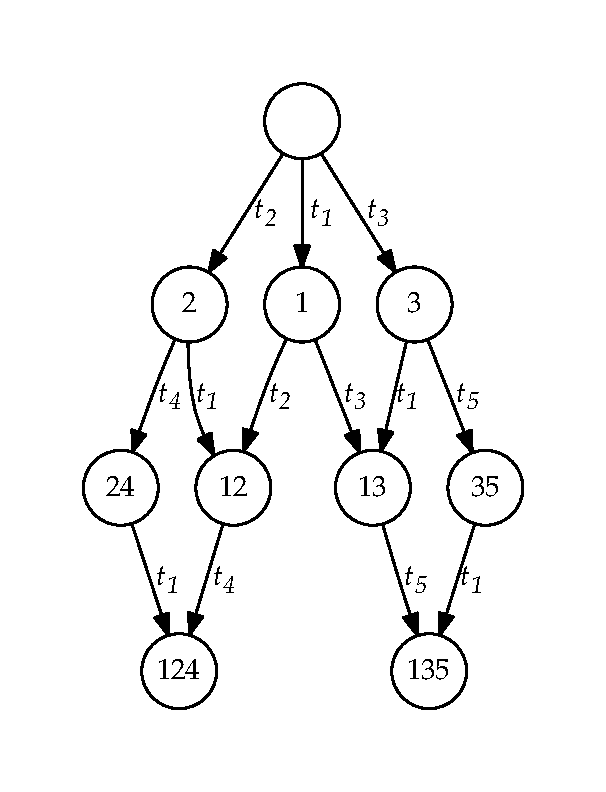
\includegraphics[height=9cm]{persistent1}
	\caption{Diagram of an example state space, for
		the illustration of persistent sets.}
	\label{fig:persistent}
\end{figure}

For illustration, in the state space shown in
figure~\ref{fig:persistent}, $T = \{t_1\}$ is
a persistent set in the initial state, as each
transition reachable following only transitions
not in $T$ is independent with $t_1$.
Likewise, $T = \{t_2, t_3\}$ is
a persistent set in the initial state, as the
only transition reachable from the initial state
without executing any transitions in $T$ is $t_1$,
and $t_1$ is independent with both $t_2$ and $t_3$.
However, $T = \{t_2\}$ is not a persistent set in the
initial state, as $t_2$ and $t_3$ are not independent.
As we might hope, if we choose only transitions
in a persistent set (either $\{t_1\}$ or $\{t_2, t_3\}$)
from the initial state to begin
an otherwise exhaustive search of the state space, then
both stopped states are reachable.

Indeed, it can be shown that if a stopped state is reachable by an exhaustive
search of the state space, then by computing a persistent set $T$ at
each state $\sigma$ and exploring only those transitions from
$\sigma$ that are in $T$, that stopped state is still reachable
(cf. Theorem 4.3 in \textbf{Godefroid thesis}). It can also be shown
that by exploring only transitions in persistent sets, all reachable
local states of each process are explored (cf. Theorem 6.14 in
\textbf{Godefroid thesis}). Therefore, if we are interested in
the definition of model checking given in 
section~\ref{sec:simple-model-checking}, then it is sufficient
to explore transitions from the persistent sets of the states we
encounter.

\subsubsection{Sleep Sets}

Another technique for addressing the state explosion
problem is that of \emph{sleep sets}. Suppose that
we are at state $\sigma_0$ when performing a search
of the state space (see figure~\ref{fig:sleep}).
Suppose that the first transition
we explore is $t_1$, reaching $\sigma_1$,
and the second is $t_2$, reaching $\sigma_2$.
If $t_1$ and $t_2$ are independent, then there
is a state $\sigma'$ reachable by both
$\sigma \xrightarrow{t_1} \sigma_1
\xrightarrow{t_2} \sigma'$ and
$\sigma \xrightarrow{t_2} \sigma_2
\xrightarrow{t_1} \sigma'$.
Any stopped state reachable from $\sigma'$
is reachable from $\sigma_1$, as $\sigma_1$
is reachable from $\sigma'$. By assumption,
when the search is at $\sigma_2$, we have already
explored all the stopped states reachable from
$\sigma_1$ (the dotted area in figure~\ref{fig:sleep}),
in particular those reachable from
$\sigma'$. Therefore, there is no need to
explore $t_1$ from $\sigma_2$.

In fact, there is no need to consider executing
$t_1$ in our recursive exploration from $\sigma_2$
until we execute some transition $t'$ which is
\emph{not} independent of $t_1$, as after
the execution of $t'$, exploring $t_1$ may
now lead to an unexplored area of the state space.

A \emph{sleep set} for a particular state
is then the set of transitions which, when
explored, is guaranteed by the above
argument to lead to an already-explored
section of the state space. The technique of
sleep sets is orthogonal to the technique
of persistent sets -- there is no interaction
between the two techniques, so implementing
both simultaneously can be achieved with
no extra difficulty.

\begin{figure}[h]
	\centering
	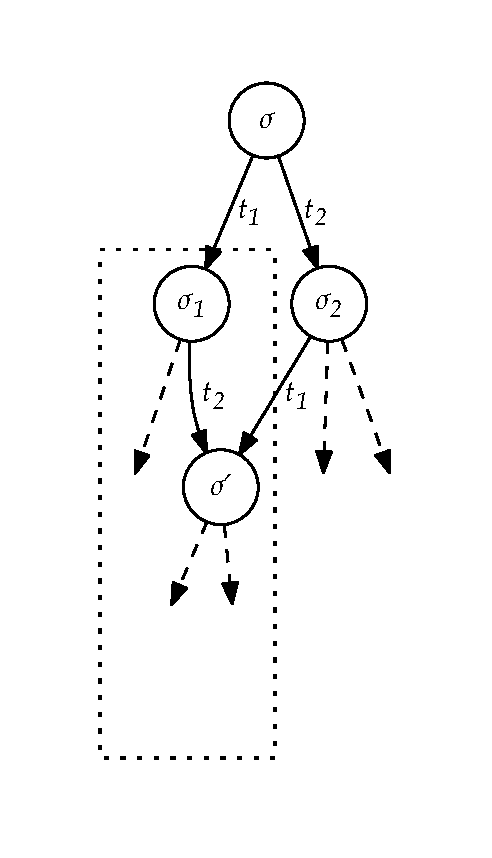
\includegraphics[height=8cm]{sleep}
	\caption{Diagram illustrating of the theory
		of sleep sets.}
	\label{fig:sleep}
\end{figure}

\section{Dynamic Partial-Order Reduction}
\textbf{This section introduces the DPOR
	algorithm, which is the main algorithm
	of the project.	
	Is this the best place for it?}

\subsection{Definitions}

\subsubsection{Transition Sequences}
Instead of keeping track of just the current state, as
the algorithms in section~\ref{sec:simple-model-checking}
did, the DPOR algorithm keeps track of a \emph{transition
sequence} $\pi \in \mathcal{T}^*$. This transition
sequence is implicitly executed from the initial state of
the transition system, $\sigma_0$, so that in practice,
$\pi = t_0, t_1, \ldots, t_{n-1}$ specifies a sequence of states
$\sigma_0, \sigma_1, \ldots, \sigma_n$ such that
\[
	\sigma_0 \xrightarrow{\ t_0\ } \sigma_1 \xrightarrow{\ t_1\ }
	\ldots \xrightarrow{t_{n-1}} \sigma_n.
\]

Given a transition sequence $\pi = t_0, t_1, \ldots, t_{n-1}$,
we use the following notation:
\begin{itemize}[label={}]
	\newcommand{\defsindent}{3.5em}
	\item{\makebox[\defsindent]{\hfill$\pi_i$}
		--- the transition $t_i$;}
	\item{\makebox[\defsindent]{\hfill$\pi.t$}
		--- the transition sequence $\pi$ extended with
		an additional transition $t$;}
	\item{\makebox[\defsindent]{\hfill$\textit{dom}(\pi)$}
		--- the set $\{i \in \mathbb{N} \mid 0 \leq i < n \}$;}
	\item{\makebox[\defsindent]{\hfill$\textit{pre}(\pi, i)$}
		--- the state $\sigma_i$ (i.e. the state before transition $t_i$); and}
	\item{\makebox[\defsindent]{\hfill$\textit{last}(\pi)$}
		--- the state $\sigma_n$.}
\end{itemize}

\subsubsection{The Happens-Before Relations}\label{sec:happens-before}

Suppose that two adjacent transitions, $\pi_i$ and $\pi_{i+1}$,
are swapped in a
transition sequence, $\pi$, to give a new
transition sequence, $\pi'$. Suppose further
that $\pi_i$ and $\pi_{i+1}$ are independent.

Since $\pi_{i+1}$ is enabled in $\textit{pre}(\pi, i+1)$,
$\pi_{i+1}$ must also be enabled in $\textit{pre}(\pi, i)$,
by the first condition of independence
(cf. section~\ref{sec:independence}). If $\pi_{i+1}$
is executed in $\textit{pre}(\pi, i)$ (as we now know
it can be), it results in a state in which $\pi_i$
can be executed, again by the first condition of
independence.

By the second
condition of independence, the state reached by
executing $\pi_i$ followed by $\pi_{i+1}$ is the same
as the state reached by executing $\pi_{i+1}$ followed
by $\pi_i$.
So $\textit{pre}(\pi, i+2) = \textit{pre}(\pi', i+2)$. Since 
for all $j \geq i + 2$, $\pi_j = \pi'_j$, it follows that
$\textit{last}(\pi) = \textit{last}(\pi')$.

Such equivalent interleavings
of transitions are precisely what we're interested in.
We can think of a transition sequence as representing
the equivalence class of transition sequences obtained
by swapping adjacent pairs of independent transitions;
if we can identify that two transition sequences are
members of the same equivalence class, we need only
explore one.

To help us to reason about such equivalence classes,
we will use a ``happens-before" relation to identify
when one transition cannot be swapped with another.
In particular, we define the \emph{happens-before}
relation $\longrightarrow_\pi$ for a transition
sequence $\pi$ to be the smallest relation on
$\textit{dom}(\pi)$ such that
\begin{enumerate}
	\item if $i \leq j$ and $\pi_i$ is dependent with
		$\pi_j$ then $i \longrightarrow_\pi j$; and
	\item $\longrightarrow_\pi$ is transitively closed.
\end{enumerate}

By construction, the happens-before relation is a
partial-order relation on the transitions in $\pi$,
and $\pi$ is one of the linearisations of this
partial order. The other linearisations of the
partial order are the equivalent sequences of
transitions which can be obtained by swapping
adjacent pairs of independent transitions in $\pi$.

In DPOR, we will also use a variant of the
happens-before relation to determine when
backtracking points are needed. Formally, 
if $i \in \textit{dom}(\pi)$ and $p \in
\mathcal{P}$ then we
say that $(i, p)\!\hookrightarrow_\pi$ if
either
\begin{enumerate}
	\item $\textit{proc}(\pi_i) = p$; or
	\item $\exists k \in \{k \ in \mathbb{N} \mid i < k < n\}.\;
		i \longrightarrow_\pi k \wedge \textit{proc}(\pi_k) = p$.
\end{enumerate}
Informally, if $(i, p)\!\hookrightarrow_\pi$ then
in every linearisation $\hat{\pi}$ of the
happens-before relation (i.e. every sequence
obtained by swapping pairs of adjacent and
independent transitions in $\pi$), then the next
transition that process $p$ executes in
state $\textit{pre}(\pi, i)$ is executed
at some point before $\textit{last}(\hat{\pi})$.

\subsection{The Algorithm}

\begin{figure}
		\begin{algorithmic}[1]
			\Procedure{Explore}{$\pi$}
			\Let{$\sigma$}{$\textit{last}(\pi)$}
			\ForAll{$p \in \mathcal{P}$}
			\Let{$R_1$}{$\{i \in \textit{dom}(\pi) \mid
				\pi_i \text{ is dependent with } \textit{next}(\pi, p)\}$}
			\Let{$R_2$}{$\{i \in R_1 \mid
				\pi_i \text{ may be co-enabled with } \textit{next}(\pi, p)\}$}
			\Let{$R_3$}{$\{i \in R_2 \mid (i, p)\!\not \hookrightarrow_\pi\}$}
			\If{$R_3 \neq \emptyset$}
			\Let{$i$}{$\text{max}(R_3)$}
			\Let{$E$}{$\{q \in \textit{enabled}(\textit{pre}(\pi, i)) \mid
				q = p \vee \exists j \in \textit{dom}(\pi).\; j > i \wedge
				q = \textit{proc}(\pi_j) \wedge (j, p)\hookrightarrow_\pi
				\}$}
			\If{$E \neq \emptyset$}
			add any $q \in E$ to $\textit{backtrack}(\textit{pre}(\pi, i))$
			\Else {
				add all $q \in \textit{enabled}(\textit{pre}(\pi, i))$
				to $\textit{backtrack}(\textit{pre}(\pi, i))$
			} \EndIf
			\EndIf
			\EndFor
			\If{$\exists p \in \textit{enabled}(\pi)$}
			\Let{$p$}{any $p \in \textit{enabled}(\pi)$}
			\Let{$\textit{backtrack}(\sigma)$}{$\{p\}$}
			\Let{$\textit{done}(\sigma)$}{$\emptyset$}
			\While{$\exists q \in (\textit{backtrack}(\sigma)\setminus\textit{done}(\sigma))$}
			\Let{$\pi'$}{$\pi.\textit{next}(\sigma,q)$}
			\State $\textsc{Explore}(\pi')$
			\State add $q$ to $\textit{done}(\sigma)$
			\EndWhile
			\EndIf
			\EndProcedure
			\State
			\State Initially: $\textsc{Explore}(\emptyset)$
		\end{algorithmic}
	\caption{The DPOR algorithm}
	\label{dpor-outline} 
\end{figure}


\chapter{Implementation}
\textbf{This chapter explains how the mathematical
	psuedocode in the literature was translated
	into a working program which model checks a
	given source file.}

\section{Design of the Software}

The project was implemented in OCaml, which
offers a few key advantages:
\begin{itemize}
	\item a clean, functional
	style, which is particularly appropriate for
	this project, given its mathematical nature;
	\item a strong, safe type system, which makes
	impossible a large class of runtime errors;
	\item parametric polymorphism, a module system,
	and other higher-order programming features,
	facilitating abstraction and generalisation; and
	\item established libraries, providing efficient
	implementations of basic data structures and algorithms.
\end{itemize}
I took particular advantage of the module system when
designing and implementing the project. OCaml modules
are used to encapsulate related definitions and hide
information -- \emph{signatures} are software interfaces
providing declarations,
and \emph{structures} are implementations which 
provide definitions. A structure \emph{matches} a
signature if it has a definition for each declaration
in the signature. \emph{Functors} can be thought of
as functions from structures to structures. If a
module matches a given signatures, then it can be
passed to a functor to give a new structure.

\begin{figure}
	\centering
	\begin{subfigure}{.4\textwidth}
		\centering
		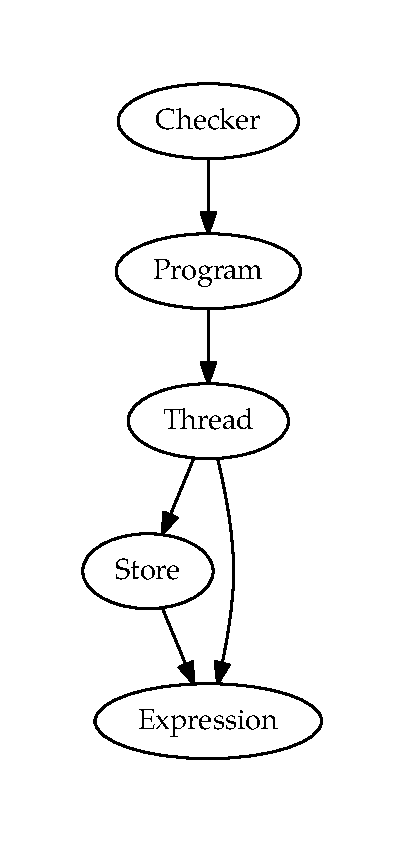
\includegraphics[height=9cm]{interfaces}
		\caption{Diagram showing which signatures declare
			which other signatures as nested sub-structures.}
		\label{fig:interfaces}
	\end{subfigure}%
	\quad
	\begin{subfigure}{.5\textwidth}
		\centering
		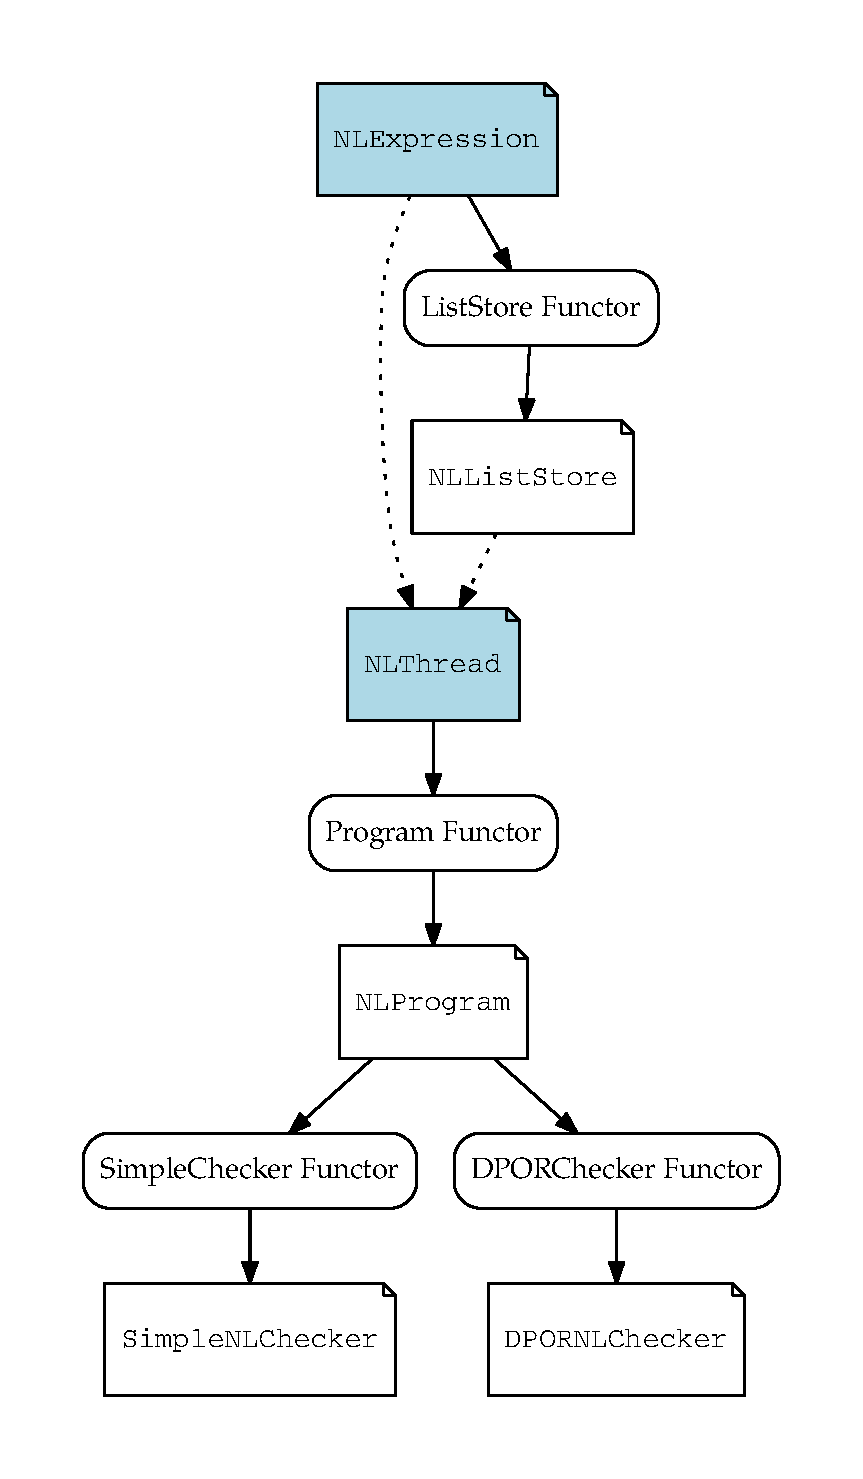
\includegraphics[height=12cm]{functors}
		\caption{Diagram showing generation of
			structures using functors. The blue files must be provided;
			the functors are part of this project; the remaining files
			are generated using the functors.}
		\label{fig:functors}
	\end{subfigure}
	\caption{Diagrams showing the interactions between
		the software modules.}
	\label{fig:design}
\end{figure}

In the project, there are five main signatures:
\begin{enumerate}
	\item a structure that matches \emph{Expression}
	contains information about the structure of expressions
	in the programming language of interest;
	\item a structure that matches \emph{Store}
	implements a store (i.e. a mapping from locations
	to expressions) for some implementation of \emph{Expression};
	\item a structure that matches \emph{Thread} contains
	the information about the semantics of expressions
	for a programming language;
	\item a structure that matches \emph{Program}
	contains declarations relating to
	transition systems as expressed in some programming
	language; and
	\item a structure that matches \emph{Checker}
	contains a function which performs model checking.
\end{enumerate}

While I did implement a simple programming language
(see section~\ref{sec:language}), the model checking
algorithms that are the focus of this project are of
course entirely independent of any particular language.
I therefore ensured that, in order to use
my project to perform model checking for programs
in any other language, the work that would have to
be done would be minimal. In particular, given implementations
of \emph{Expression} and \emph{Thread} (effectively
specifying the semantics of a programming language), my system uses
functors to automatically generate implementations of
\emph{Store}, \emph{Program} and \emph{Checker}, the
last of which can then be used to immediately perform
model checking. This process is shown explicitly in
figure~\ref{fig:functors}.

\section{Development of Project Language}\label{sec:language}
\textbf{This section explains how I designed
	and implemented the language in which the
	concurrent programs to be model checked
	are written.}

\subsection{Language Design}
\textbf{First, the language had to be designed.
	Explain design choices, give sense of what
	the language is, maybe an example program,
	and point to the appendix for a full definition.}

Although, as mentioned above, any programming language
could be used to express transition systems for model
checking, I chose to design and implement a simple
ML-like language, PL (Project Language), to avoid
the unnecessary complexity of implementing a full
industrial language.
The grammar for valid PL expressions is given in
figure~\ref{fig:pl-expressions}.

\begin{figure}
	\centering
	\setlength{\tabcolsep}{2pt}
	\begin{tabular}{rl}
		\textit{expr} $:=$ & \textit{int} $\vert$ \textit{bool} $\vert$ \textit{var} \\
		$\vert$ & \textit{local} $\vert$ \textit{global}
			$\vert$ \textit{spinlock} \\ 
		$\vert$ & \textit{expr op expr} $\vert$ $\neg\,$\textit{expr} \\
		$\vert$ & \textbf{skip} $\vert$ \textit{expr; expr}\\
		$\vert$ & \textbf{if} \textit{expr}
			\textbf{then} \textit{expr} \textbf{else} \textit{expr} \\
		$\vert$ & \textbf{while} \textit{expr}
			\textbf{do} \textit{expr} \\
		$\vert$ & \textit{expr} $:=$ \textit{expr} $\vert$ !\textit{expr} 
			$\vert$ \textbf{ref} \textit{expr} \\
		$\vert$ & \textbf{fn} \textit{var}
			$\Rightarrow$ \textit{expr} $\vert$ \textit{expr expr} \\
		$\vert$ & \textbf{let} \textit{var} $=$
			\textit{expr} \textbf{in} \textit{expr} \\
		$\vert$ & \textbf{let rec} \textit{var} $=$
			\textbf{fn} \textit{var} $\Rightarrow$
			\textit{expr} \textbf{in} \textit{expr} \\
		$\vert$ & \textbf{lock} \textit{expr} $\vert$
			\textbf{unlock} \textit{expr} \\
		$\vert$ & \textbf{cas}(\textit{expr}, \textit{expr}, \textit{expr}) \\
		$\vert$ & \textbf{error}(\textit{message}) \\
		& \\
		\textit{int} $\in$ & $\{\ldots, -1, 0, 1, \ldots\}$ \\
		\textit{bool} $\in$ & $\{\textbf{true}, \textbf{false}\}$ \\
		\textit{var} $\in$ & \textit{Variable}
	\end{tabular}
	\qquad\quad
	\begin{tabular}{rcl}
		\textit{op} $:=$ & $+$ &\\
		$\vert$ & $-$ &\\
		$\vert$ & $\ast$ &\\
		$\vert$ & $/$ &\\
		$\vert$ & $\%$ &\\
		$\vert$ & $>$ &\\
		$\vert$ & $<$ &\\
		$\vert$ & $=$ &\\
		$\vert$ & $\&$ &\\
		$\vert$ & $\mid$ &\\
		& &\\
		\textit{local} & $\in$ & \textit{Location} \\
		\textit{global} & $\in$ & \textit{Location} \\
		\textit{spinlock} & $\in$ & \textit{Location} \\
		& &\\
		\textit{Location} & $=$ & $\{a, b, c, \ldots\}^\ast$\\
		\textit{Variable} & $=$& $\{x, y, z, \ldots\}$ \\
	\end{tabular}
	\caption{The grammar for PL expressions.}
	\label{fig:pl-expressions}
\end{figure}

As required by the \emph{Thread} interface, each
PL thread has access to both its local store $s$
and the global store $g$. Both $s$ and $g$ are
maps from locations to expressions.
To express the semantics
of PL, then, we need to give whether or not an
expression $e$ reduces for local store $s$ and
global store $g$, and if it does, we need to give
the expression $e'$ that it reduces to in one ``step",
as well as any updates to $s$ and $g$ that result.
Note that each such ``step" is assumed to be atomic.
The semantics of PL expressions are as you would expect
(see \textbf{THE APPENDIX} for a full definition), but
the rules for the reduction of expressions that interact
with the global store $g$ are given in figure~\ref{fig:pl-rules}.

\begin{figure}
	\begin{gather*}
		\frac{g(\textit{spin}) = \textbf{true}}
			{(\textbf{unlock}\ \textit{spin},\ s,\ g)
				\longrightarrow (\textbf{skip},\ s,\
				g[\textit{spin} \mapsto \textbf{false}])} \\
		\\
		\frac{g(\textit{spin}) = \textbf{false}}
		{(\textbf{lock}\ \textit{spin},\ s,\ g)
			\longrightarrow (\textbf{skip},\ s,\
			g[\textit{spin} \mapsto \textbf{true}])} \\
		\\
		\frac{g(\textit{glob}) = e_\textit{curr}}
			 {(\textbf{cas}(\textit{glob},\, e_\textit{curr},\, e_\textit{new})
			 	,\ s,\ g) \longrightarrow (\textbf{true},\ s,
			 	\ g[\textit{glob} \mapsto e_\textit{new}])} \\
		\\
		\frac{g(\textit{glob}) \neq e_\textit{curr}}
			{(\textbf{cas}(\textit{glob},\, e_\textit{curr},\, e_\textit{new})
				,\ s,\ g) \longrightarrow
				(\textbf{false},\ s,\ g)} 
	\end{gather*}
	\caption{Rules for the atomic reduction of PL
		expressions that interact with the shared store.}
	\label{fig:pl-rules}
\end{figure}

There is no type system for PL. Although it would have been
beneficial to design and implement a type system for PL
(a type checker could catch type errors early, rather than a runtime
failure with non-obvious causes occurring), I thought that the total
time I would have spent on creating the type system would be more than
the time taken in dealing with the problems resulting from having
no type system. With the benefit of hindsight, I think this was the
correct decision.

\subsection{Parser}
On the other hand, I decided that investing time in creating a
parser for PL would pay itself off over the course of the project.
This allows me to write, for example,
\begin{align*}
	\texttt{let y = ref 1 in cas(Gx, 7 * !y - 3, 0)},
\end{align*}
instead of having to type the OCaml meta-language abstract
syntax tree representing the structure of the Pl expression:
\begin{align*}
	\texttt{Let (Ref (Integer}& \texttt{ 1), Cas (Global "x",
		Op (Op (Integer 7,} \\ \texttt{Mult,}& \texttt{ Deref (Var 0)), Minus, Integer 3),
		Integer 0))}.
\end{align*}
Writing such expressions is not only extremely time-consuming but
also error-prone. For the language to be of any practical use,
a parser is a necessity.

To create a parser for PL, two program generators were used:
\emph{OCamllex} and \emph{Menhir}. When presented with a
file giving a mapping from strings of characters to tokens,
OCamllex produces a lexical analyser, which converts a sequence
of characters into a sequence of tokens. When presented with a
grammar and a set of precedence rules, Menhir produces a parser,
which converts a sequence of tokens into an abstract syntax tree
of the grammar. These were used in conjunction, as shown in
figure~\ref{fig:parsing}, to produce a PL parser.

\begin{figure}
	\centering
	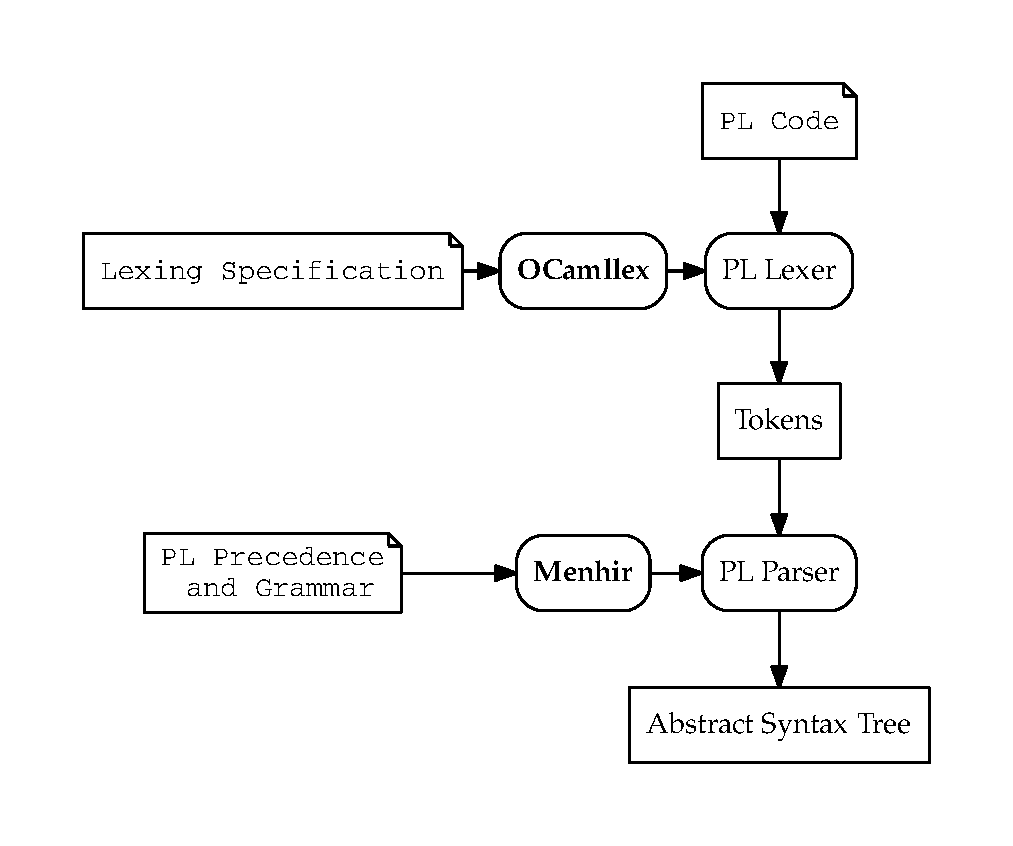
\includegraphics[height=10cm]{parsing}
	\caption{Diagram showing the flow and processing of
		information in the generation of a PL abstract
		syntax tree.}
	\label{fig:parsing}
\end{figure}

\subsection{Implementation}

\subsubsection{The Expression Module}
There are actually two datatypes which are used to
represent PL expressions in the
PL implementation of the \emph{Expression} module.
The first of these is the ``raw" expression, which
uses strings to represent variables (this is the
datatype that the parser produces). However,
manipulation of expressions is much easier when
variables are represented using \emph{de Bruijn indices},
which is the purpose of the second expression datatype.
This is the only one required by the \emph{Expression}
signature. A function exists to recursively convert
from the ``raw" datatype to this second datatype.

The remainder of the \emph{Expression} module
consists of auxiliary functions, which are
necessary for the implementation of later
modules, and either return a simple piece
of information or perform a simple manipulation.

\subsubsection{The Store Module}
As mentioned above, I implemented a functor
called \textbf{ListStore}, which, given a structure
matching the \emph{Expression} signature,
gives a structure matching the \emph{Store}
signature. The \emph{Store} implementation produced
represents stores using a simple list of
(location, expression) pairs. If a location
appears twice in the list, the occurrence
nearest the head of the list is taken to be
the correct value. A function is provided
which walks through from head to tail and
removes any stale pairs, which although
linear in time, reduces the space taken
by the list.

More efficient store implementations are of
course possible (for example, one based on
a hash table rather than a list), but
I went for the simplest reasonable
implementation I could think of, to
ensure correctness.

The only other function of note is
\texttt{get\char`_fresh\char`_loc},
which queries the \emph{Expression} \texttt{random\char`_loc}
function until it returns a result which is
unbound in the store. This is used to generate a location
to use when a new local reference is created using the
\textbf{ref} keyword.

\subsubsection{The Thread Module}
The \emph{Thread} module consists mostly of
the \texttt{next\char`_step} and \texttt{next\char`_transition}
functions. The \texttt{next\char`_step} function uses pattern
matching on PL expressions to determine what the next atomic
operation, if any, to be executed in the reduction
of the expression is. There is a close correspondence
between the
rules of the operational semantics (see \textbf{APPENDIX})
and the different cases in the pattern matching. This is
because each rule specifies that an expression of a
particular form, perhaps with some conditions on the
states of the local and shared stores, reduces in a
particular way. For illustration, one rule and its
corresponding pattern matching case is shown in 
figure~\ref{fig:step-rule-correspondence}.

\begin{figure}
	\begin{subfigure}{\textwidth}
		\begin{gather*}
		\frac{}
		{(\textbf{if true then } e_2 \textbf{ else }
				e_3,\,s,\,g) \rightarrow (e_2,\,s,\,g)}
		\qquad
		\frac{}
		{(\textbf{if false then } e_2 \textbf{ else }
			e_3,\,s,\,g) \rightarrow (e_3,\,s,\,g)} \\
		\\
		\frac{(e_1,\,s,\,g) \rightarrow
			(e_1^{\prime},\,s^{\prime},\,g^{\prime})}
		{(\textbf{if } e_1 \textbf{ then }
			e_2 \textbf{ else } e_3,\,s,\,g)
			\rightarrow (\textbf{if } e_1^{\prime}
			 \textbf{ then }
			e_2 \textbf{ else } e_3,\,
			s^{\prime},\,g^{\prime})}
		\end{gather*}
		\caption{Rules relating to
			the reduction of if-then-else expressions.}
	\end{subfigure}
	\\ \\ \\
	\begin{subfigure}{\textwidth}
		\lstinputlisting[frame=none, firstline=59, lastline=63]
			{../src/pl_thread.ml}
		\caption{Pattern matching case for if-then-else expressions.
			If \texttt{e1} is a Boolean, then reduce to \texttt{e2} or
			\texttt{e3},
			otherwise use a recursive call to try to reduce \texttt{e1}.}
	\end{subfigure}
	\caption{A concrete illustration of the correspondence
		between the rules of the operational semantics
		and the pattern matching statements of the
		\texttt{next\char`_step} function.}
	\label{fig:step-rule-correspondence}
\end{figure}

As a transition for a thread is defined as a
finite sequence of \emph{invisible} local
operations, followed by one \emph{visible} operation
which accesses the shared store, the \texttt{next\char`_transition}
function simply repeatedly calls the \texttt{next\char`_step}
function, reducing the initial expression and modifying
the local store, until either the resulting step accesses the shared
store, or no further reduction is possible. Noting that this
process is independent of the object language (PL, in this case),
the most general implementation of this project would require
only the  \texttt{next\char`_step} function to be provided by
the user, with a functor being used to automatically
produce the \texttt{next\char`_transition} function. However,
in this case, I decided that the additional design complexity
cost was not worth the slight improvement to the abstraction
of the project.

\subsubsection{The Program Module}
The \emph{Program} module is a small functor which,
when given a \emph{Thread} implementation, provides 
the few additional definitions and auxiliary
functions necessary to fully represent
transition systems (cf. section~\ref{sec:background-defs}.)
In particular, a state $\sigma \in \textit{State}$ is
represented by an instance of the \texttt{state} type:
\lstinputlisting[frame=none, firstline=107, lastline=107]
	{../src/interfaces.ml}

\subsubsection{Testing}
To ensure that the implementation of the PL
language was correct, I wrote unit tests for
the \texttt{next\char`_transition} and
\texttt{next\char`_step} functions. These tests
consisted of a series of inputs and expected outputs
to these functions. My aim in writing these tests
was to ensure that most of the code was covered,
so that any obvious bugs could be corrected
immediately. However, I did not invest time
making these tests very rigorous for two reasons:
any bugs found later would be relatively straightforward
to correct; and getting the PL implementation
fully correct was not the aim of the project, but
just a necessary step before the main work on the
model checking algorithms.


\section{Simple Model Checker}

In order to ensure the correctness of my implementation
of the DPOR algorithm, to have a baseline to use
for performance comparison, and to reaffirm my understanding
of the implementation of model checking, I first wrote the
SimpleChecker functor, which takes an implementation of
\emph{Program} as its input, and outputs a structure
which includes the definition of
a function that performs model checking by performing
an exhaustive depth-first search of the state space --
the simplest possible model checking algorithm.

Include why \texttt{check local} was put in Thread.

\subsection{Implementation}
\begin{itemize}
	\item Functor from programs to Checkers (independent of language)
	\item Present pseudo-code which is fairly close to OCaml but
		without too much detail.
	\item In particular explain how errors and deadlocks are found
	\item Aim is to convince reader that definitely correctly
		implemented.
\end{itemize}

\subsection{Testing}
\begin{itemize}
	\item Some test cases to sanity check
	\item In practice did error first and deadlock later,
		but not super relevant
	\item Idea is to use this to check DPOR, because this is so 
		obviously correct
\end{itemize}

\section{Dynamic Partial-Order Reduction}
\textbf{This section explains how the DPOR
	alogorithm was implemented in practice.}

\subsection{Implementation}
\subsubsection{Clock Vectors}
\textbf{Used to decide the happens-before relation.}
\subsubsection{Independence}
\textbf{Keep track of last transition that accessed
	each global object.}

\subsection{Locks}
\textbf{Difficulties faced adding locks;
	how they were overcome.}

Problem: many algorithms use locks. While \texttt{while locked do skip done}
is good enough, it results in a cycle in the state space, which causes
non-termination of DPOR.

Solution: add locks. New problem: no distinction between
transition not existing and not being enabled. Without
locks, all existing transitions were enabled; no longer
the case.

Solution: pass around Boolean stating whether or not the transition
is enabled.

\section{Stateful Model Checking}
\textbf{Keeping track of already-visited states.}

\subsection{Simple Model Checker}
\textbf{Straight-forward implementation for simple
	checker. Give new algorithm.}

When searching through state space, the same state is often
re-encountered. Idea: keep track of visited states, and don't bother
re-exploring from those we have already explored.

\subsection{Dynamic Partial-Order Reduction}
\textbf{Applying ideas to DPOR. Why na\"{i}ve
	approach doesn't work; the solution.}

\subsubsection{Na\"{\i}ve Approach}
\textbf{What this approach is; why it doesn't
	work; example.}

The same approach can be applied to
the DPOR algorithm -- whenever we
encounter a state from which we have already
explored, return immediately because we
already know the result. However, this
na\"ive algorithm is unfortunately unsound.

\subsubsection{Stateful Dynamic Partial-Order Reduction}
\textbf{Present SDPOR algorithm.}

Idea: conservatively add in necessary points to backtrack sets.
Use visible operation dependency graph.

\section{Sleep Sets}
\textbf{Implementation of sleep
	sets in both the simple checker
	and in DPOR.}
\subsection{Simple Model Checker}
\subsection{DPOR}

\section{Counter-Example Traces}

One of the advantages of model checking as
a formal method is that, in the case that
an error is found, it is trivial to give
an example of an execution of the given
program which leads to an error state; in
our case, this is just the sequence of
transitions executed at the point when
an error state it found.

To give more insight into the reason for the
error state being entered, it would be preferable
to instead present the use with a
\emph{partial order} of the transitions which,
whenever any linearisation of the partial order
is executed, results in the error/deadlock state.
Given a sequence of transitions which lead to
some error state, the problem is
then to give the most general partial order
which, however linearised, results a sequence
of transitions 

This partial order is just the happens-before
relation (cf. \ref{sec:happens-before}). As
discussed above  (\textbf{where?}), this can
be decided using clock vectors.
Just execute the transition sequence
from the beginning, keeping track of the relation.
Then output it in a nice form, so we can display it
as a graph maybe.

\begin{figure}	
	\lstinputlisting[firstline=39,lastline=57]{prog.ml}
	\caption{The function giving the partial order from
		a given transition sequence.}
\end{figure}

\chapter{Evaluation}
\textbf{This chapter presents evidence
	for the correctness of the
	algorithm implementations in the
	project, and evaluates their
	performance.}

\section{Soundness}
\textbf{This section gives references
	proving the soundness of the underlying
	algorithm, then gives evidence that my
	implementation is a sound implementation
	of the theoretical algorithm.}

\textbf{Is it best to be honest about the
	possibility of incorrectness, or just
	to persuade that everything is sound?}

\subsection{PL Interpreter}
\subsection{Simple Model Checker}
\subsection{DPOR}
\subsection{Stateful Checking}
\subsubsection{Simple}
\subsubsection{DPOR}
\subsection{Sleep Sets}
\subsection{Counter-Example Traces}

\section{Performance}
\textbf{This section compares the
	performance of the various algorithms
	in the project. This is achieved by
	looking at execution times, transitions
	explored, and numbers of states explored
	while model checking various example
	programs. Comparison can be made with
	published figures.}

\chapter{Conclusions}

\textbf{This chapter makes some
	interesting conclusions, which I
	haven't thought of yet.}


%%%%%%%%%%%%%%%%%%%%%%%%%%%%%%%%%%%%%%%%%%%%%%%%%%%%%%%%%%%%%%%%%%%%%
% the bibliography
\addcontentsline{toc}{chapter}{Bibliography}
\bibliography{refs}

%%%%%%%%%%%%%%%%%%%%%%%%%%%%%%%%%%%%%%%%%%%%%%%%%%%%%%%%%%%%%%%%%%%%%
% the appendices
\appendix

\chapter{PL Definition}
 
\textbf{This will be the definition
	of PL.}
 
\chapter{Example PL Programs}

\textbf{This will contain various
	example programs, in particular
	those used for performance evaluation.}

\chapter{Project Proposal}

Project proposal here
% \input{proposal_without_title}

\end{document}
